\documentclass[12pt]{article}
\usepackage[utf8]{inputenc}
\usepackage[spanish]{babel}
\usepackage{graphicx}
\usepackage{hyperref}
\hypersetup{
    colorlinks=true,
    linkcolor=cyan,
    filecolor=magenta,      
    urlcolor=blue,
    }

\title{CAFETERIA\\\emph{Menu}}
\author{Victor Chavarria, Samuel Gutierrez, Jonathan Zavala, Grecia Morales}
\date{Septiembre, 2023}

\begin{document}

\maketitle

\newpage
\tableofcontents
\newpage

\section {REQUERIMIENTOS FUNCIONALES}

\subsection {Cliente}
\begin{itemize}
  \item Seleccionar categorias.
	\item Seleccionar la comida.
	\item Revisar el pedido.
	\item Selecciona complementos al pedido.
	\item Confirmar pedido.
	\item Editar pedido.
	\item Editar cantidades de items.
	\item Obtener turno.
	\item Guardar turno en dispositivo.
	\item Recibir notificaciones del estado del pedido.
	\item Regresar al menu.
\end{itemize}

\subsection {Recepcionista}
\begin{itemize}
	\item Recibe el pedido del cliente.
	\item Liga el turno/pedido del cliente con la mesa disponible.
\end{itemize}

\subsection {Cocina}
\begin{itemize}
	\item Recibe el pedido.
	\item Selecciona el  pedido.
	\item Marcar pedido como completado.
	\item Notificar que el pedido ya est� listo.
\end{itemize}

\section {REQUERIMIENTO NO FUNCIONAL}
\begin{itemize}
  \item Desarrollo en VSC.
	\item Framework Cake php.
	\item Uso de internet para la app.
	\item Acceso al carrete (Guardado del pedido).
	\item Acceso a las notificaciones (estado de los pedidos).
\end{itemize}

\newpage
\section {CASOS DE USO:}
\subsection {Diagrama}
\begin{figure}[htbp]
	\centering
		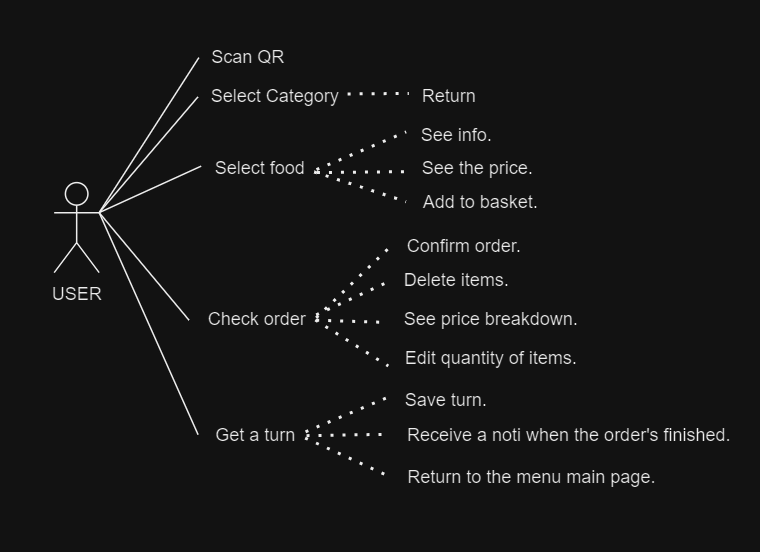
\includegraphics[width=1.00\textwidth]{C:/Users/victo/Documents/Repositories/Amerike/3rdSemester/Cafeteria-Menu/Assets/Img/DiagramaCasos/Diagrama-casos-user.png}
	\caption{Diagrama de casos usuario}
	\label{fig:Diagrama-casos-user}
\end{figure}

\begin{figure}[htbp]
	\centering
		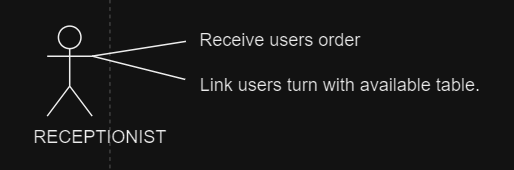
\includegraphics[width=1.00\textwidth]{C:/Users/victo/Documents/Repositories/Amerike/3rdSemester/Cafeteria-Menu/Assets/Img/DiagramaCasos/Diagrama-casos-receptionist.png}
	\caption{Diagrama de casos recepcionista}
	\label{fig:Diagrama-casos-receptionist}
\end{figure}

\begin{figure}[htbp]
	\centering
		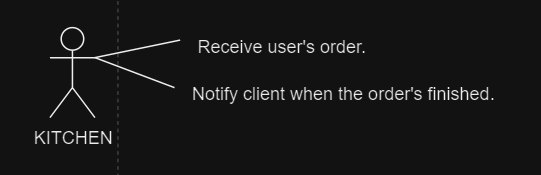
\includegraphics[width=1.00\textwidth]{C:/Users/victo/Documents/Repositories/Amerike/3rdSemester/Cafeteria-Menu/Assets/Img/DiagramaCasos/Diagrama-casos-kitchen.png}
	\caption{Diagrama de casos cocina}
	\label{fig:Diagrama-casos-kitchen}
\end{figure}

\newpage
\subsection {Flujo ideal}
\begin{itemize}
  \item Escanear QR.
	\item LogIn / SignUp.
  \item Seleccionar una categor�a.
  \item Seleccionar un alimento.
  \item Agregar a la canasta.
	\item Revisar su pedido.
	\item Obtener tu turno.
\end{itemize}

\subsection {Flujo alterno}
\begin{itemize}
	\item Escanear QR.
	\item LogIn / SignUp.
  \item Seleccionar una categor�a.
		\subitem Revisar tu canasta.
  \item Seleccionar un alimento.
		\subitem Revisar la informaci�n del alimento.
		\subitem Agregar el alimento a la canasta.
		\subitem Revisar la canasta.
		\subitem Regresar a la selecci�n de categor�as.
  \item Revisar pedido.
		\subitem Regresar a la selecci�n de categor�as.
		\subitem Confirmar pedido.
		\subitem Editar cantidades de item.
		\subitem Eliminar items.
	\item Obtener tu turno.
		\subitem Guardar turno en carrete.
		\subitem Regresar al menu.
\end{itemize}

\newpage
\section {DIAGRAMAS}
\subsection {Diagrama de componentes}
\begin{figure}[htbp]
	\centering
		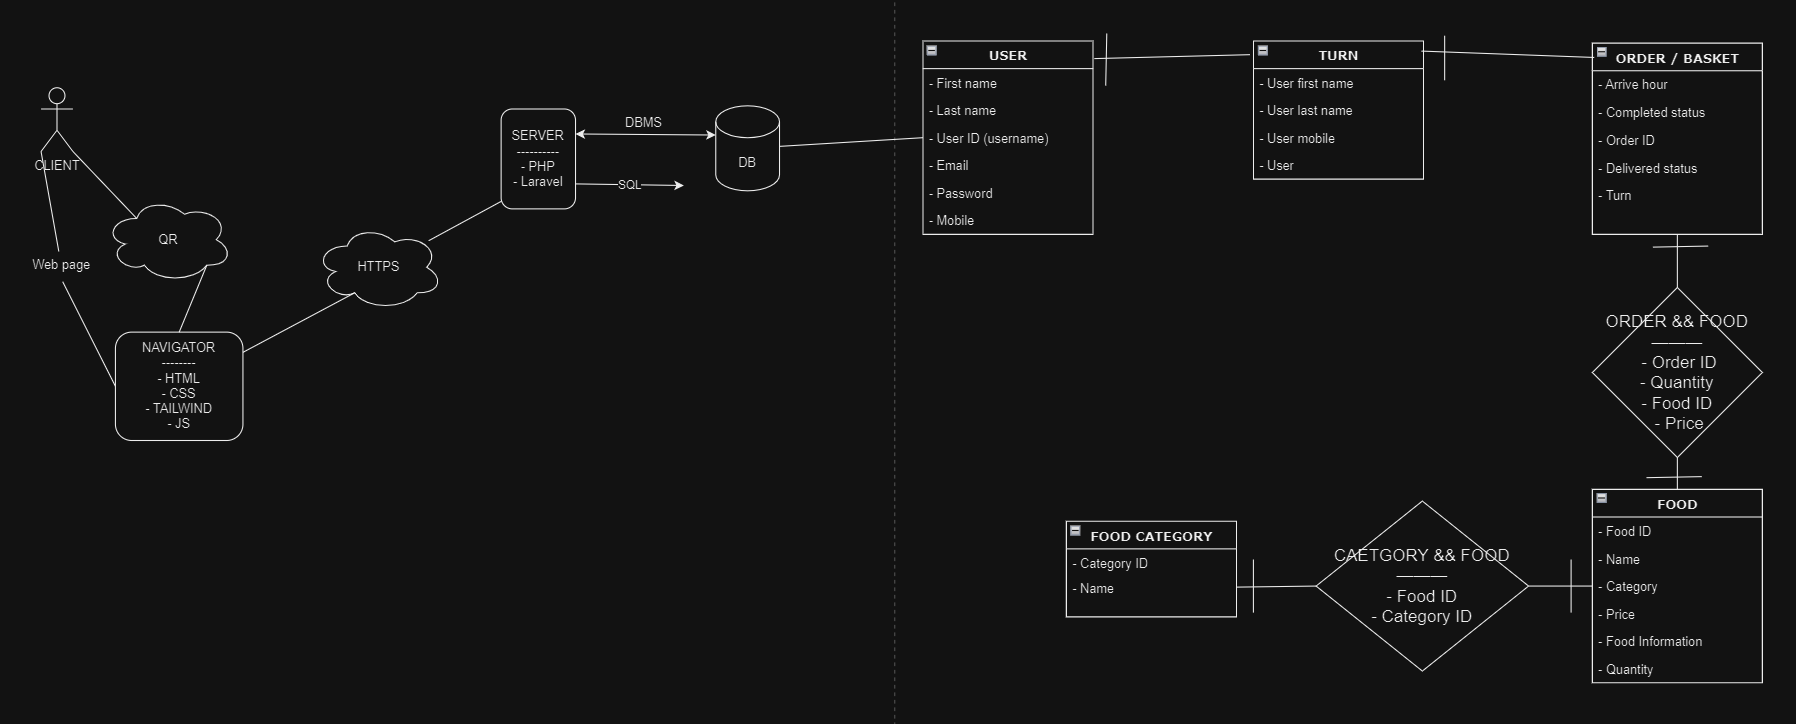
\includegraphics[width=1.00\textwidth]{C:/Users/victo/Documents/Repositories/Amerike/3rdSemester/Cafeteria-Menu/Assets/Img/DiagramaComponentes/Diagrama-componentes-general.png}
	\caption{Diagrama de componentes}
	\label{fig:Diagrama-componentes-general}
\end{figure}

\subsection {Diagrama de clases}
\begin{figure}[htbp]
	\centering
		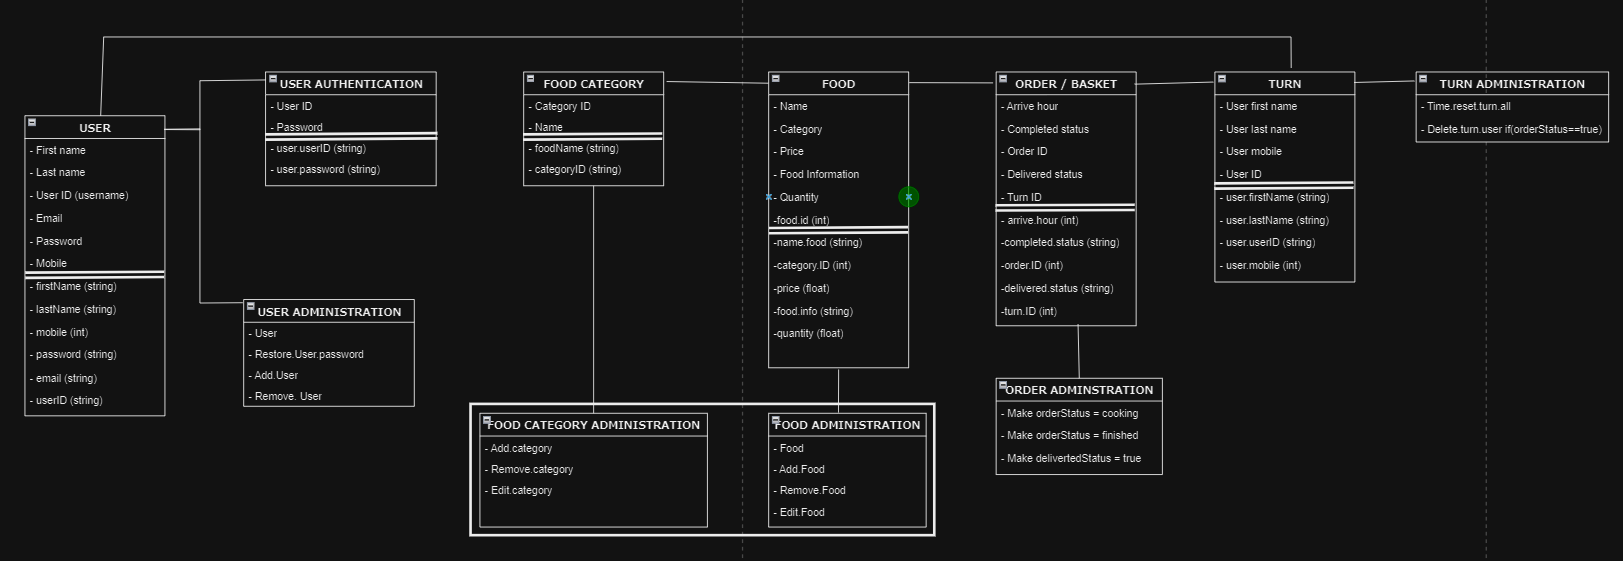
\includegraphics[width=1.00\textwidth]{C:/Users/victo/Documents/Repositories/Amerike/3rdSemester/Cafeteria-Menu/Assets/Img/DiagramaClases/Diagrama-clases-general.png}
	\caption{Diagrama de clases}
	\label{fig:Diagrama-clases-general}
\end{figure}

\newpage
\subsection {Diagrama de secuencia}
\begin{figure}[htbp]
	\centering
		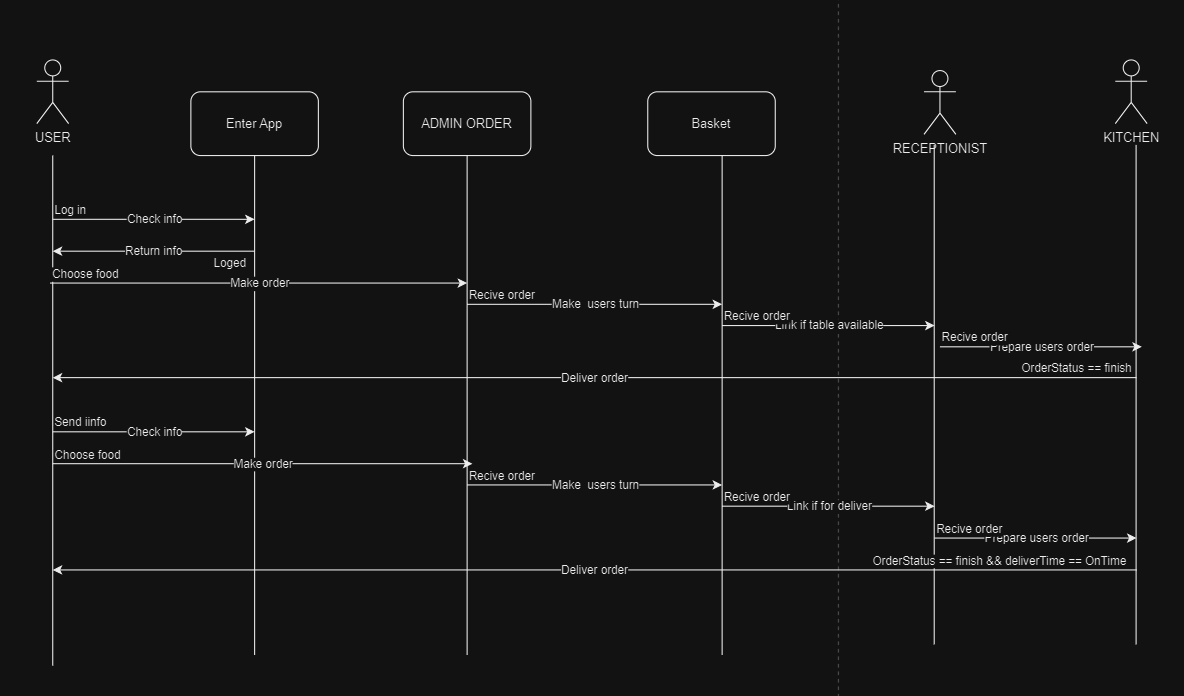
\includegraphics[width=1.00\textwidth]{C:/Users/victo/Documents/Repositories/Amerike/3rdSemester/Cafeteria-Menu/Assets/Img/DiagramaSecuencia/Diagrama-secuencia-general.png}
	\caption{Diagrama de secuencia general}
	\label{fig:Diagrama-secuencia-general}
\end{figure}

\begin{figure}[htbp]
	\centering
		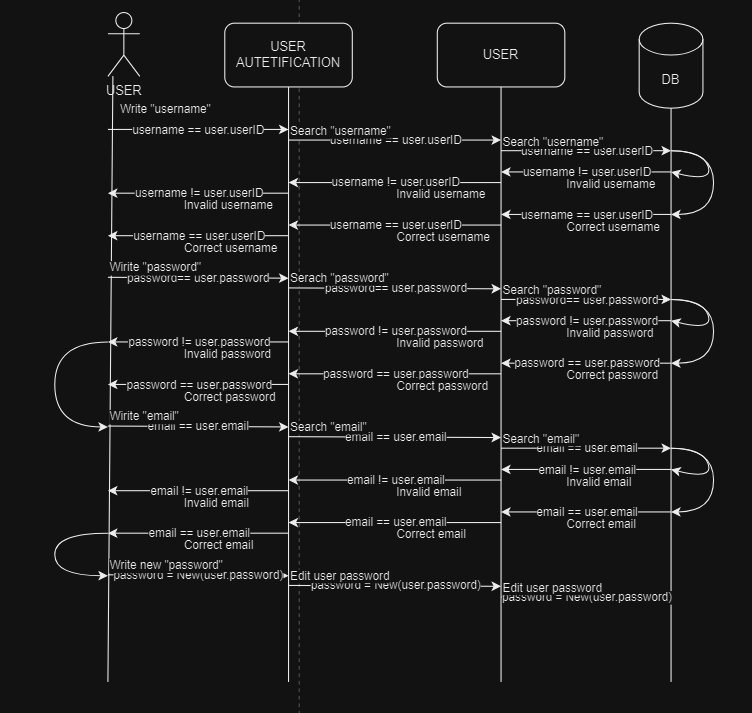
\includegraphics[width=1.00\textwidth]{C:/Users/victo/Documents/Repositories/Amerike/3rdSemester/Cafeteria-Menu/Assets/Img/DiagramaSecuencia/Diagrama-secuencia-LogIn.png}
	\caption{Diagrama secuencia LogIn}
	\label{fig:Diagrama-secuencia-LogIn}
\end{figure}

\begin{figure}[htbp]
	\centering
		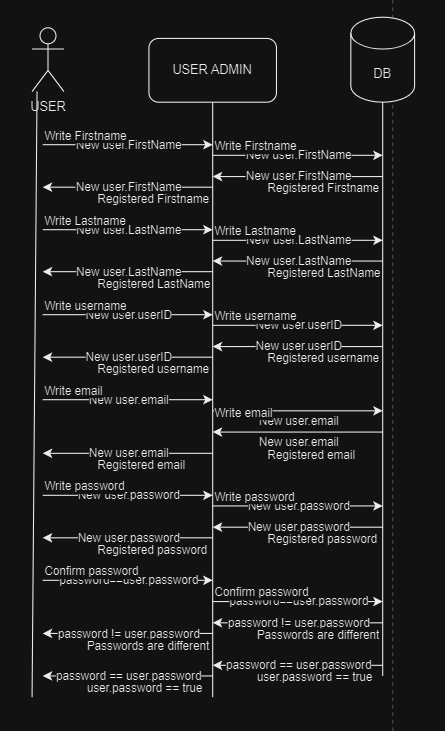
\includegraphics[width=0.80\textwidth]{C:/Users/victo/Documents/Repositories/Amerike/3rdSemester/Cafeteria-Menu/Assets/Img/DiagramaSecuencia/Diagrama-secuencia-SignUp.png}
	\caption{Diagrama secuencia SignUp}
	\label{fig:Diagrama-secuencia-SignUp}
\end{figure}

\begin{figure}[htbp]
	\centering
		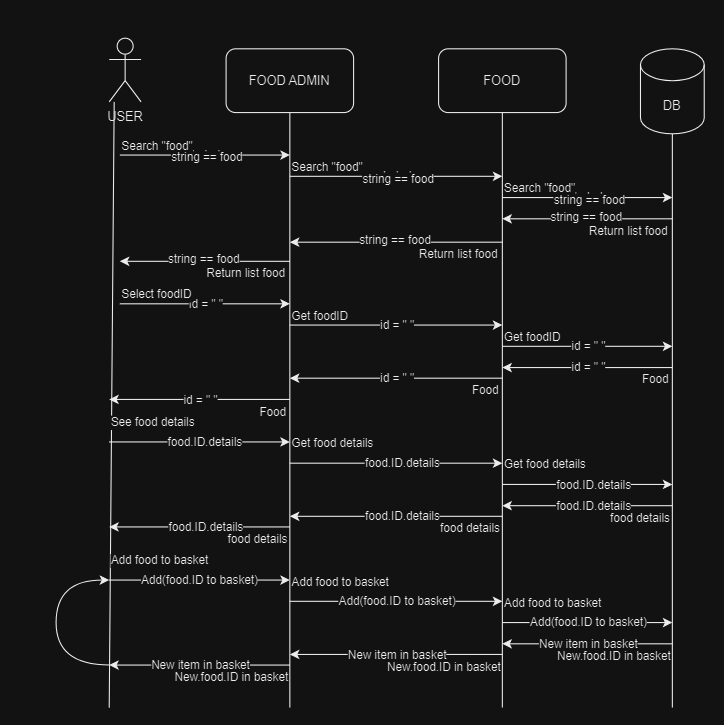
\includegraphics[width=1.00\textwidth]{C:/Users/victo/Documents/Repositories/Amerike/3rdSemester/Cafeteria-Menu/Assets/Img/DiagramaSecuencia/Diagrama-secuencia-agregar-comida.png}
	\caption{Diagrama secuencia pedir comida}
	\label{fig:Diagrama-secuencia-agregar-comida}
\end{figure}

\begin{figure}[htbp]
	\centering
		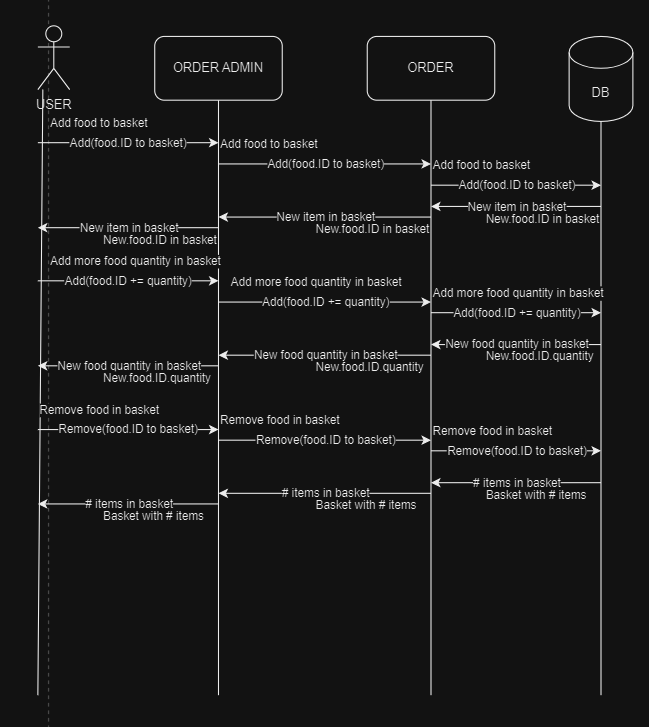
\includegraphics[width=1.00\textwidth]{C:/Users/victo/Documents/Repositories/Amerike/3rdSemester/Cafeteria-Menu/Assets/Img/DiagramaSecuencia/Diagrama-secuencia-orders.png}
	\caption{Diagrama secuencia ordenes}
	\label{fig:Diagrama-secuencia-orders}
\end{figure}


\end{document}